\section{Conclusion}

This design failed to be completed. Reexamining the plan of design for this project reveals a few issues that made effective implementation difficult. Planning on a lack of delay communication between hardware modules creates a significant amount of planning difficulty. Every module's input and output speed must be able to be predetermined and buffers (which understand how to handle delays) added. This can result in the use of numerous overly large buffers due to worse case calculations being used to determine the buffer size. Additionally, this plan is made more difficult by multiple 802.16 frames being pushed through the same hardware one after the other. As the number of outputted bits (prior to conversion to wide Q and I signals) is larger than the number of inputted bits, a delay between frame inputs from outside the system or a buffer of infinite size is required. Clearly, infinite flip-flops are not a possibility in any logic circuit, thus the system as a whole would need an understanding of when it was "ready" for more data.

Further along the same track, the current design does not allow for the use of internal modules for separate frames simultaneously. For example, the reed-Solomon encoder cannot be easily used for one frame while the convolution coder begins processing the next. One possible plan to allow this to be done simply is to have a signal between modules for when a frame begins or ends (rather than using a central piece of logic to manage this). Unfortunately, we need more than just knowledge of when the frame begins and ends to properly process it; a whole slew of metadata needs to be passed along while being timed properly with the motion of the bitstream through the system. Additionally this metadata would need to handle delays properly (as using solely buffering is unfeasible). From these requirements, the possibility of using a second bitstream to carry the metadata arises, as shown in \autoref{fig:alt-bitstream}. Each module could stay as initially designed, but be wrapped in a controller which handles extraction of metadata from the bitstream as well as properly handling it's timing. It could be passed along ahead of the start of a frame such that when the actual data reaches a new module, the necessary metadata for processing it is already present. Of course, additional issues arise if the metadata bitstream can exceed the length of the shortest 802.16 frame: an additional delay would need to be inserted after a short frame to give time for the metadata to be transferred.

Using an FPGA for this is probably not economically viable or efficient. Power consumption would be much higher than could be achieved with a non-FPGA realization. Cost would also be an issue for any product with a non-inconsequential volume of production. As wireless devices are often  mobile and battery powered, power consumption is a serious concern. Additionally, using this as portion of a larger FPGA design would not be feasible due to the high use of logic circuit resources by various components, primarily the (planned) IFFT.


\begin{figure}
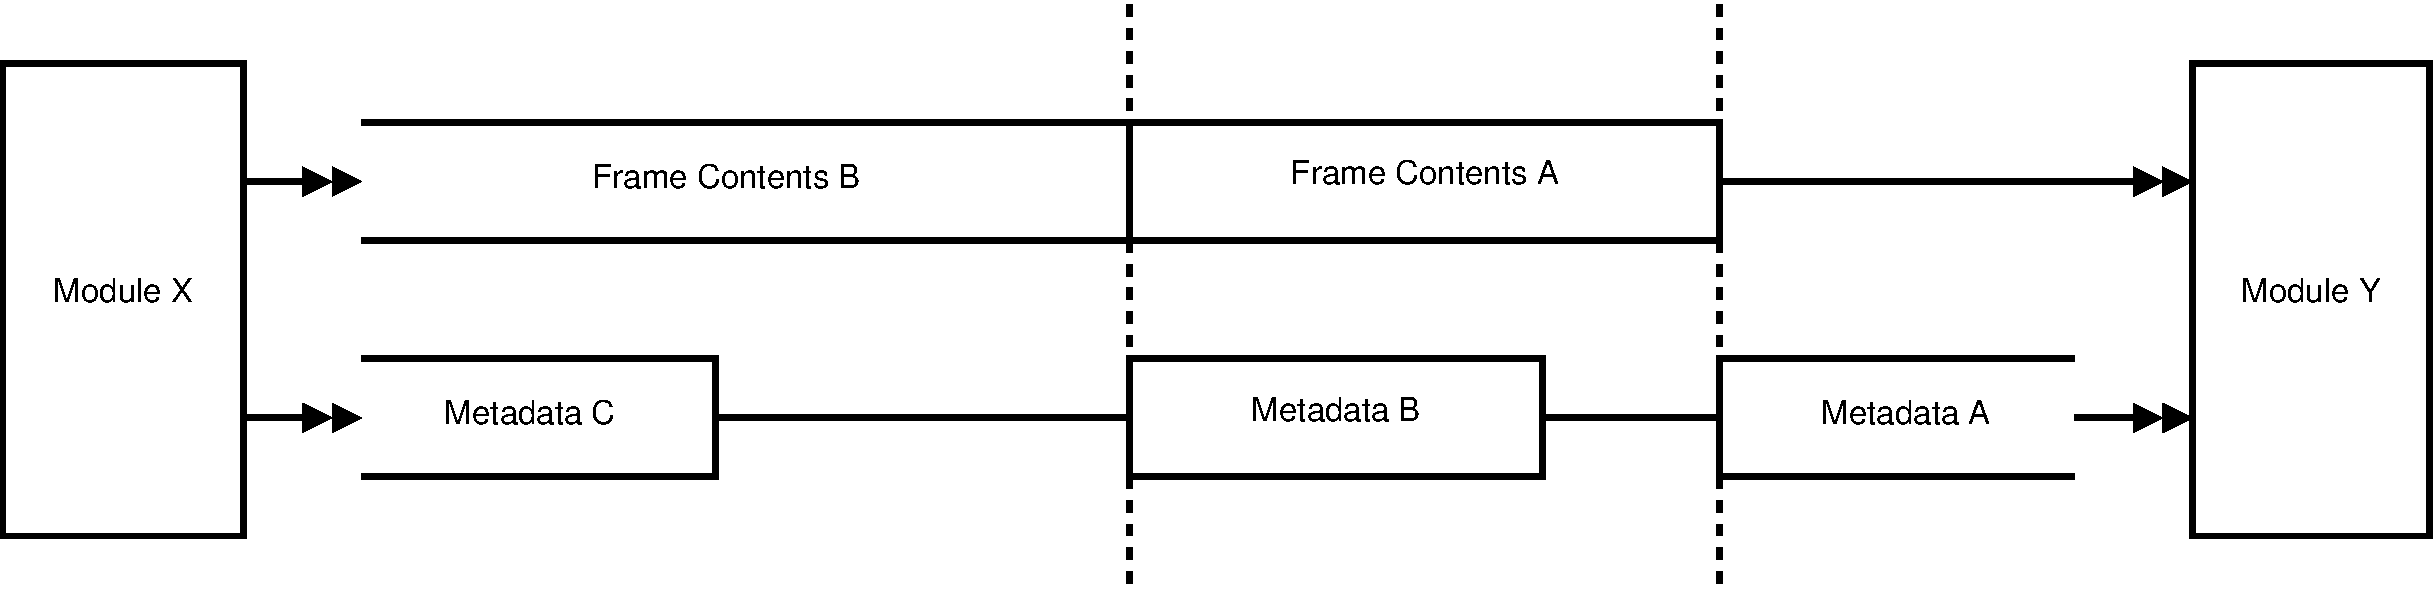
\includegraphics[width=\linewidth]{conclution_metadata_transfer}
\caption{Proposed Bitstream Transfer Pattern	}
\label{fig:alt-bitstream}
\end{figure}
